\documentclass[12pt]{scrbook}
\usepackage{geometry}
\usepackage{graphicx}
\usepackage{import}
\usepackage{xcolor}
\usepackage{listings}
\usepackage{caption}
\usepackage{hyperref}
\usepackage{tikz}
\usetikzlibrary{calc,positioning,shapes.geometric}

\geometry{a4paper}
\setlength{\parindent}{0pt}

\DeclareCaptionFormat{listing}{\colorbox{black!15}
  {\parbox{5cm}{#1#2#3}}}
\captionsetup[lstlisting]{format=listing,
%labelfont=white,textfont=white,
singlelinecheck=false, margin=0pt, font={bf,footnotesize}}

\newcommand{\OpenPEARL}{\textit{OpenPEARL}}

\begin{document}
\title{\OpenPEARL{} - Inter Module Checker (imc)}

\author{R. M\"uller}

\lstnewenvironment{XMLCode} {
    \lstset{numbers=left,
            title={XML},
            frame=tlrb,
            breaklines = true,
            belowcaptionskip=4pt
    }
}%
{}%

\lstnewenvironment{CppCode} {
    \lstset{numbers=left,
            title={C++},
            frame=tlrb,
            breaklines = true,
            belowcaptionskip=4pt
    }
}%
{}%

\lstnewenvironment{PEARLCode} {
    \lstset{numbers=left,
            title={PEARL},
            frame=tlrb,
            breaklines = true,
            belowcaptionskip=4pt
    }
}%
{}%
\pagestyle{myheadings}
\markboth {\OpenPEARL{} imc \today} {\OpenPEARL{} imc \today}

\date{
ToDo:
\begin{itemize}
\item check, whether array of dations, signals or interrupts are possible
\item investigate about parameters in REF DATION
\item how to enshure proper mapping of REF DATIONS in STRUCTs
\end{itemize}
}

\maketitle

\tableofcontents

\chapter{Introduction}
A PEARL program consists of several separatly compilable modules.
The interface between the modules is defined by SPC and DCL statements with the
attribute GLOBAL.
The declaration of plattform dependent elements like INTERRUPTs, 
DATIONs and SIGNALs must be done in the SYSTEM-part.

For proper operation the types of the specified and declared elements must
fit. 
For system elements, we need a mechanism to obtain the type in an
extensible way. This is solved by the use of an interface definition as 
xml-file for each system element.

This tool checks all global definitions and specifications and checks for
\begin{itemize}
\item proper types, including the types of system elements
\item multiple declarations
\item missing declarations
\item unused declarations
\end{itemize}

\section{Structure}
As shown in \cite{mueller2016} the structure of operation of the \OpenPEARL{}
compilation system is like:
\newcommand*\circled[1]{\tikz[baseline=(char.base)]{
   \node[shape=circle,fill=white,draw,minimum size = 0.5cm, inner sep=2pt] (char) {#1};}}

\begin{figure}[bpht]

  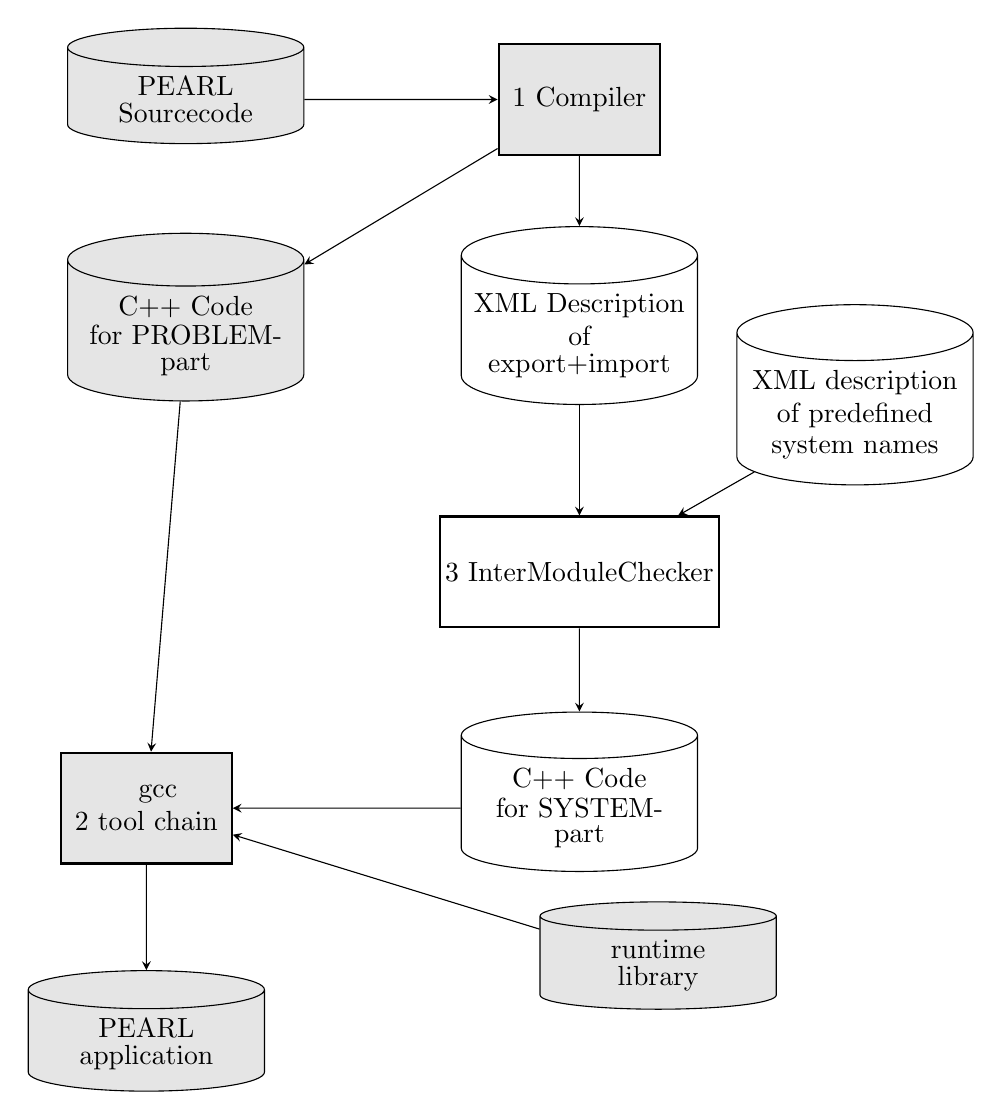
\begin{tikzpicture}[
    >=stealth,
    node distance=3.5cm,
    file/.style={
      cylinder,
      cylinder uses custom fill,
      %cylinder body fill=yellow!50,
      %cylinder end fill=yellow!50,
      shape border rotate=90,
      minimum width=3cm,
      aspect=0.25,
      draw
    },
        fileold/.style={
          cylinder,
          cylinder uses custom fill,
          cylinder body fill=gray!20,
          cylinder end fill=gray!20,
          shape border rotate=90,
          minimum width=3cm,
          aspect=0.25,
          draw
        },
    block/.style = { rectangle,
    				draw=black,
    				 thick, 
                    %fill=blue!20,
                    text centered, minimum width=5em,
                    %rounded corners,
                    inner sep = 2pt,
                    minimum height=4em },
    blockold/.style = { rectangle,
       				draw=black,
       				 thick, 
                       fill=gray!20,
                       text centered, minimum width=5em,
                       %rounded corners,
                       inner sep = 0.5em,
                       minimum height=4em }                          
  ]
    \node[fileold] (prl) at (0,10) {\shortstack{PEARL\\Sourcecode}};
    \node[blockold] (sprachumsetzer) at (5,10) {\circled{1} Compiler};
    \node[fileold,below of=prl,yshift=0.5cm] (problemcc) {\shortstack{C++ Code\\for PROBLEM-\\part}};
    \node[file,below of=sprachumsetzer,yshift=0.5cm] (modulxml) {\shortstack{XML Description
                                                            \\of \\
                                                             export+import}};
    \draw[->] (prl) -- (sprachumsetzer);
    \draw[->] (sprachumsetzer) -- (problemcc);
    \draw[->] (sprachumsetzer) -- (modulxml);

    \node[file, yshift=-1cm,right of=modulxml] (hardwarexml) {\shortstack{XML description \\of predefined\\system names}};
    \node[block, below of=modulxml,yshift=0.5cm] (imc) {\circled{3} InterModuleChecker};

    \draw [->] (modulxml) --  (imc);
    \draw [->] (hardwarexml) -- (imc);
    
    \node[file, below of=imc,yshift=0.5cm] (systemcc) {\shortstack{C++ Code\\ for SYSTEM- \\part}};
    \node[fileold, below of=systemcc, yshift=1.5cm, xshift=1cm] (runtimelib) {\shortstack{runtime\\library}};
    \node[blockold, left of=systemcc,xshift=-2cm] (gcc)
    {\circled{2}
    {\shortstack{gcc\\tool chain}}};
    \draw[->] (imc) -- (systemcc);
    \draw[->] (systemcc) -- (gcc);
    \draw[->] (runtimelib) -- (gcc);
    \draw[->] (problemcc) -- (gcc);
    
    \node[fileold, below of=gcc,yshift=0.5cm] (pearlapp) {\shortstack{PEARL\\application}};
    \draw[->] (gcc) -- (pearlapp);
  \end{tikzpicture}
\caption{Structure of the \OpenPEARL{} build system.}
\label{aufbau}
\end{figure}



The first stage compiler creates an C++-representation of the PEARL-module
together with an xml-representation of the export and import interface.

The definition of system names may be done by the user to order to supply 
additional system devices.
Each system name must be accompanied by the developer with a xml-representation
of the system element. The imc tool extracts the required information
from these xml-files and verifies a proper system configuration.

\section{Credits}
This tool  was influenced by the master thesis of 
Stephan Hertig \cite{msc_hertwig} and the semester project of
M.Bauer, T-Schaz, J.Weber, T.Welte and J.Wirth \cite{openpearlss16}.



\chapter{Structure of Module Import and Export Definition}

The compiler creates an xml-file per PEARL-module containing the
\begin{itemize}
\item system part information
\item problem part specifications and declarations
\end{itemize}

\section{XML-Document Structure}
The compiler has no knowledges about the nature of a system name.
Thus the system part is translated as it is --- only syntactical errors
are recognized. 
The document has the root tag \verb|<module>|, which hat the attribute
\verb|file| with the value source file name.  
All system elements are in the xml-subtree \verb|<system>|.
All problem part elements with attribute GLOBAL are located
in the xml-subtree \verb|problem|.

\begin{XMLCode}
<?xml version="1.0" encoding="UTF-8" ?>
<module file="demo.prl">
<system>
   <username .... >
   ....
   </username>
   <configuration .... >
   ....
   </configuration>
</system>
<problem>
  <spc .../>
  <dcl .../>
  ...
</problem>
</module>
\end{XMLCode}

\section{System Part Elements}
\subsection{User Names \texttt{<username>}}
If a system element defines a user name the \verb|<username>| tag is 
used. Each user name is accompanied by an system name with the tag 
\verb|<sysname>|, which may have parameters.
Maybe there is a list of associations, thus there may by a tree
of \verb|<association>| tags.
The user name tag contains the attribute \verb|line| with the value of the 
source code line number.

\subsection{System Name \texttt{<sysname>}}
\label{sec_system_names}
The system name tag contains the attribute \verb|name| containing the 
name of the system element.

\subsection{Parameters \texttt{<parameters>}}
The parameters are located in the \verb|<parameters>|-subtree.
The imc tool supports constants of type FIXED, CHAR and BIT.
The compiler detects  the type of the parameter
from the literal and passes the literal as content to the corresponding
\verb|<FIXED>|-, \verb|<CHAR>|- or \verb|<BIT>|-tag.

\subsection{Associations \texttt{<associations>}}
An association may be ether a system name (with parameters) or a user name.
The  \verb|<association>|-tag contains the attribute \verb|name| with the 
given name as value. If parameters are specified for the association,
they are passed as \verb|<parameters>|-subtree in the same way as decribed 
in section \label{sec_system_names}.

There is no check in the compilation phase necessary,
whether a name is a system name
or a user supplied name.


\subsection{Configuration Item}
Configuration elements in the system part are located in the
\verb|<configuration>|-element. 
The only difference to the \verb|<username>|-tag is the absence of the 
\verb|name|-attribute. Parameters and associations apply identical.

\subsection{Example for System Part Elements and their Specifications}
\begin{PEARLCode}
MODULE(demo);

SYSTEM;
lm75: LM75('48'B4) --- I2CBus('/dev/i2c-0', 100000);

lm75a : LM75('49'B4) --- i2cbus1;
i2cbus1: I2CBus('/dev/i2c-1', 100000);

sig1: FixedRangeSignal;
int1: UnixSignal(15);

disc: Disc('/tmp/folder1', 10);

stdOut: StdOut;

Log('EW') --- StdOut;

PROBLEM,
SPC sig1 SIGNAL GLOBAL;
SPC int1 INTERRUPT GLOBAL;
SPC disc DATION OUT DIRECT SYSTEM ALL GLOBAL;
SPC stdOut DATION OUT SYSTEM ALPHIC GLOBAL;
SPC lm75 DATION IN SYSTEM FIXED(15) GLOBAL;

MODEND;
\end{PEARLCode}

\begin{XMLCode}
<?xml version="1.0" encoding="UTF-8" ?>
<module file="demo.prl">
<system>
   <username name="lm75" line="4">
      <sysname name="LM75">
      <parameters>
         <BIT>'48'B4</BIT>
      </parameters>
   </sysname>
   <association name="I2CBus">
      <parameters>
         <CHAR>'/dev/i2c-0'</CHAR>
         <FIXED>100000</FIXED>
      </parameters>
   </association>
</username>

<username name="lm75a" line="6">
   <sysname name="LM75">
      <parameters>
         <BIT>'49'B4</BIT>
      </parameters>
   </sysname>
   <association name="i2cbus1">
   </association>
</username>

<username name="i2cbus1" line="7">
   <sysname name="I2CBus">
      <parameters>
         <CHAR>'/dev/i2c-1'</CHAR>
         <FIXED>100000</FIXED>
      </parameters>
   </sysname>
</username>

<username name="sig1" line="9">
   <sysname name="FixedRangeSignal"/>
</username>

<username name="int1" line="10">
   <sysname name="UnixSignal">
      <parameters>
         <FIXED>15</FIXED>
      </parameters>
   </sysname>
</username>

<username name="disc" line="12">
   <sysname name="Disc">
      <parameters>
         <CHAR>'/tmp/folder1'</CHAR>
         <FIXED>10</FIXED>
      </parameters>
   </sysname>
</username>

<username name="stdOut" line="14">
   <sysname name="StdOut">
   </sysname>
</username> 

<configuration line="16">
   <sysname name="Log">
      <parameters>
         <CHAR>'EW'</CHAR>
      </parameters>
   </sysname>
   <association name="StdOut">
   </association>
</configuration>
</system>
<problem>
<spc type="signal" name="sig1" line="19"/>
<spc type="interrupt" name="int1" line="20" />
<spc type="dation" name="disc" line="21">
   <attributes> OUT,SYSTEM, DIRECT </attributes>
   <data>ALL</data>
</spc>
<spc type="dation" name="stdOut" line="22">
      <attributes> OUT, SYSTEM </attributes>
      <data>ALPHIC</data>
</spc>
<spc type="dation" name="lm75" line="23">
      <attributes> IN, SYSTEM </attributes>
      <data>A15</data>
</spc>
</problem>
</module>
\end{XMLCode}
\section{Problem Part Elements}
\subsection{Specification of System Part Elements}
The PEARL source code defined the type of a system name to be ether a DATION, 
INTERRUPT or DATION. According detected type, the compiler 
adds a xml-tag \verb|<spc>|-tag with attributes \verb|type| anf \verb|line|
containing the value \verb|"dation"|, \verb|"interrupt"| or \verb|"signal"|,
 respectively.
While interrupts and signals have no parameters, dations need more
specifications. The attributes are stores as comma separated list in the
\verb|<attributes>|-subelement, the transmission data is given as value
of the <data>-tag. For details aboutencoding of the type information
see chapter \ref{encoding}. 

\subsection{Declaration of Problem Part Elements}

Additional type information for the \verb|type| attribute are introduced.
The additional type values are identical to the  encoding rules of
structures and structure elements  as described in \cite{runtime}.

This treats all elements except dations. They are described similar to the
system part.


\subsection{Specification of Problem Part Elements}
The specification of global  elements in the problem part are described 
in the same as their declaration.

\subsection{Example for Specification and Declarations in Problem Part}

\begin{PEARLCode}
PROBLEM;
   DCL x FIXED(7) GLOBAL;
   SPC y FIXED(17) GLOBAL;
   DCL d12 DATION OUT STRUCT [a FIXED(7), b FLOAT(53)]
     DIM(10,20)  GLOBAL CREATED(aSystemDation);
   DCL s1 SEMA PRESET(10) GLOBAL;
\end{PEARLCode}

\begin{XMLCode}
...
<problem>
  <dcl type="A7" name="x" line=".."/>
  <spc type="A15" name="y" line=".."/>
  <dcl type="dation" name="d12" line="10">
    <attributes>OUT DIM(10,20)</attributes>
    <data>S5A7B57</data>
  </dcl>
  <dcl type="I" name="s1" line="..."/>
</problem>
\end{XMLCode}


\section{Encoding of Transfer Data Types and STRUCTs}
\label{encoding}
The encoding of transfer data is like described in the runtime documentation
\cite{runtime}. The primitive data types and their length are encoded 
by a letter and an integer constant. E.g A7 is a FIXED(7). The encoding rules
for struct and arrays hold. Special values are ALL and ALPHIC.

\begin{description}
\item[ALL] fits to all data types
\item[ALPHIC] in problem part fits to ALPHIC, CHAR and ALL in system devices
\end{description}

This mapping is also used for problem part global elements, except for dations,
which need more information to be checked.

\chapter{Platform Specific Names}

\section{Introduction}
Each specific platform may support a different set of system names.
Thus each target platform is characterized by a separate xml-file.
These files are created during the build phase of the runtime system
for each target platform.

\section{Structure of the XML-File}
All possible system elements are located as unordered separate 
elements under the root tag \verb|platform|.
For the individual types of system elements, the following tags are
provided:
\begin{itemize}
\item \verb|<signal ...>| defines a system signal
\item \verb|<interrupt ...>| defines a system interupt
\item \verb|<dation ...>| defines a system dation
\item \verb|<configuration ...>| defines a configuration item
\item \verb|<connection ...>| defines a association provider, if 
   non of the above fit
\end{itemize}

These elements have attributes 
\begin{description}
\item [name] is the system name
\item [instances] the number of instances, if specified. If this attribute 
   is not specified, there is no instance limit.
\end{description}

\subsection{Signal-Tag}
The signal tag contains only the attribute \verb|name| for the
system signal name.

\subsection{Interrupt-Tag}
The interrupt tag contains the attribute \verb|name| for the
system interrupt name.
Possible parameters are listed as subtree \verb|<parameters>|.

\subsection{Dation-Tag}
The dation tag contains the attribute \verb|name| for the
system dation name.
Possible parameters are listed as subtree \verb|<parameters>|.
Possible attributes are listed as subtree \verb|<attributes>|.
Possible associations to this element are
 listed as subtree \verb|<associationProvider>|.


\subsection{Configuration-Tag}
The configuration element has the same structure as the dation tag
except the attribute \verb|name|, which has not to be present.

\subsection{Associations}
The connection between two system elements is treated by the following
elements:

\begin{itemize}
\item \verb|<needAssociation>| with the attribute 
 \verb|name| and the identifier of the expected interface. The 
  interface names are described in the runtime documentation. 
\item \verb|<associationProvider>|  with elements \verb|<associationType>|.
  Attributes for an associationType are:
  \begin{itemize}
   \item  \verb|<name>|,  which is an unique free selectable
     identifier for this kind of  association.
   \item \verb|<clients>|  if given it is the number of allowed
      clients for this connection provider. If not given, there is no
      limits of allowed clients.
   \end{itemize} 
\end{itemize}

\subsection{Parameters}
Only parameters of system elements of types bit, fixed and char are supported.
The actual value may be restricted to definite values and ranges.

Tags are defined for each of them:
\begin{itemize}
\item \verb|BIT| with the attribute \verb|length|, which specifies the 
   allowed length of an actual parameter. \verb|<BIT length="8">...</BIT>|
   specifies a BIT(8) parameter. Shorter actual parameters are extended --- 
   longer parameters induce an error message.
\item \verb|FIXED| with the attribute \verb|length|, which specifies the 
   allowed length of an actual parameter. \verb|<FIXED length="15">...</FIXED>|
   specifies a FIXED(15) parameter. Shorter actual parameters are extended --- 
   longer parameters induce an error message.
\item \verb|CHAR| with the attribute \verb|length|, which specifies the 
   allowed length of an actual parameter. \verb|<CHAR length="15">...</CHAR>|
   specifies a CHAR(15) parameter. Shorter actual parameters are allowed --- 
   longer parameters induce an error message.
\end{itemize}

Supported rules:

\begin{tabular}{|l|c|p{8cm}|}
\hline
rule & type & description \\
\hline
VALUES & BIT,FIXED, CHAR &
   a comma separated list of allowed values
   is given. Other values produce an error message. \\
\hline
NotEmpty & CHAR & 
   at least one character is required \\   
\hline
FIXEDRANGE & FIXED &
   two comma separated integers limits the allowed range
   of actual values --- borders included \\ 
\hline
FIXEDGT & FIXED &
   one integer which limits the allowed range at the low side
   of actual value --- border NOT included \\ 
\hline
\end{tabular}

\section{Sample Platform File}
\begin{XMLCode}
<?xml version="1.0" encoding="UTF-8"?>
<platform file="testPlatform.xml">
      <signal name="FixedRangeSignal"/>
      <signal name="FixedDivideByZeroSignal"/>
      <signal name="FloatIsNaNSignal"/>
      <interrupt name="UnixSignal">
         <parameters>
            <FIXED length="31">
               <VALUES>1,2,3,15,16,17</VALUES>
            </FIXED>
         </parameters>
      </interrupt>
      <dation name="Disc">
         <parameters>
            <CHAR length="32767"/>	<!-- beliebiger String -->
            <FIXED length="31">
               <FIXEDRANGE>1,9999</FIXEDRANGE>
            </FIXED>
         </parameters>
         <attributes>FORWARD, DIRECT, IN, OUT, INOUT, SYSTEM</attributes>
         <data>ALL</data>
         <associationProvider>
            <associationType name="NamedAlphicOutProvider" />
         </associationProvider>
      </dation>
      <dation name="StdIn" instances="1">
         <parameters>
         </parameters>
         <attributes>
            FORWARD, IN	, SYSTEM
         </attributes>
         <DATA>ALPHIC</DATA>
      </dation>
      <dation name="StdOut" instances="1">
         <parameters>
         </parameters>
	 <attributes>
            FORWARD, OUT, SYSTEM
         </attributes>
         <data>ALPHIC</data>
         <associationProvider>
            <associationType name="AlphicOutProvider" />
         </associationProvider>
      </dation>
      <connection name="I2CBus">
         <parameters>
            <CHAR length="32767">
               <NotEmpty />
            </CHAR>
            <FIXED length="31">	<!-- max int32_t -->
               <FIXEDGT>0</FIXEDGT>
            </FIXED>
         </parameters>
         <associationProvider>
            <associationType name="I2CBusProvider" />
         </associationProvider>
      </connection>
      <dation name="LM75">
         <parameters>
            <BIT length="8">
               <VALUES>'48'B4, '49'B4, '4A'B4, '4B'B4,
                       '4C'B4, '4D'B4 , '4E'B4, '4F'B4</VALUES>
            </BIT>
         </parameters>
         <needAssociation provider="I2CBusProvider"/>
      </dation>

  <configuration name="Log" instances="1">
    <parameters>
      <CHAR length="4">
         <NotEmpty/>
      </CHAR>
    </parameters>
    <needAssociation provider="AlphicOutProvider"/>
  </configuration>
</plattform>
\end{XMLCode}

\chapter{Usage}

\section{Invocation}
The inter module checker is invoked with
\begin{verbatim}
imc -b <target> -o <output> pearlModules...
\end{verbatim}

The option -b is  recommended. The given parameter defines the
platform definition XML file, which is expected ether in the current 
working directory (first)
or in installation directory of OpenPEARL.

The option -o defaults to system.cc in the current working directory.

The list of pearl modules is passed without extension. Pathnames are 
possible.


\section{Tests}
\subsection{Tests for System Part}
The following tests are performed for system part elements:
\begin{itemize}
\item all defined username need a predefined system name.
\item the number and type of actual parameters must fit to the 
      predefined system element
\item the value of the actual parameters are checked, if the predefined
   elements limits the parameter range
\item each used association must be supported by the specified provider
\item actual parameters of association providers must fit in type and value
   to the formal parameters, like username definitions
\item the number of association clients must agree with the supported
    number of clients
\item the number of instances of a system element does not excess the 
   allowed number of instances
\end{itemize}

\subsection{Tests for Problem Part}
The following tests are performed for problem part elements:
\begin{itemize}
\item each specified system dation, signal and interrupt must fit
  to the definition is the system part.
\end{itemize}

\subsection{Not implemented yet}
Not supported up to now:
\begin{itemize}
\item problem part global declarations and their specifications
\end{itemize}I

\section{Output}
The tool creates a C++ file for the system part if no errors are
detected. 
This file must be passed to the g++ compiler and linked with all 
other object modules.


\chapter{Documentation}

\section{Architecture}

\begin{description}
\item[Pass 1:]
The tool reads the specified xml files as DOM-trees into memory.
In case of read errors, the java default exception handling
gives information about the mistake in the input files.

\item [Pass 2:]
Scan the system part for each module and add the detected system elements
into the container \verb|SystemElements|. Forward declarations are 
recorded together with the expectation. 
Errors are created on unknown system elements, wrong number or values
of parameters. Mismatch of  associations types.
Duplicate user names are detected and reported as error.

\item[Pass 3:]
The problem part elements are checked to fit to the system definitions.
Unused defined system elements are reported as warning.

\item[Pass 4:]
The C++ source code is created.

\end{description}

The process stops after each pass, if there were errors detected.

\section{Source Code}
The source code consists of several classes, whic are documented with JavaDoc.


\begin{thebibliography}{99}
\bibitem{mueller2016}  
   M.Schaible, R. M\"uller; Konsistenzpr\"ufungen in OpenPEARL,
   In W.A. Halang, H. Unger (Hrsg.): Informatik aktuell --- 
   Internet der Dinge und Echtzeit, Springer Verlag, 2016

\bibitem{msc_hertwig}
    Stephan Hertwig: SmallPEARL ---
    Treiber f\"ur die Peripherieinfrastruktur des Raspberry,
    Masterthesis FernUNI Hagen, Sommerseemster 2015
 
\bibitem{openpearlss16}
    M.Bauer, T.Schaz, J.Weber, T. Welte, J. Wirth: OpenPEARL,
    Projektarbeit im Studiengang AIB/CNB der HS Furtwangen, Sommersemester 2016

\bibitem{runtime}
   R. M\"uller: OpenPEARL - Runtime System, Project Document

\end{thebibliography}
~                          


\end{document}
